\documentclass[conference]{IEEEtran}
\IEEEoverridecommandlockouts
\usepackage{cite}
\usepackage{amsmath,amssymb,amsfonts}
\usepackage{algorithm}
\usepackage{algorithmic}
\usepackage{graphicx}
\usepackage{textcomp}
\usepackage{xcolor}
\usepackage{booktabs}
\usepackage{array}
\usepackage{tikz}
\usetikzlibrary{arrows.meta,positioning,shapes.geometric,fit,calc,backgrounds}
\usepackage{pgfplots}
\pgfplotsset{compat=1.17}
\usepackage[hidelinks]{hyperref}
\def\BibTeX{{\rm B\kern-.05em{\sc i\kern-.025em b}\kern-.08em T\kern-.1667em\lower.7ex\hbox{E}\kern-.125emX}}

% ---------------------------------------------------------------- measured values (filled from models/eval_metrics.json)
\newcommand{\Ptot}{0.519}\newcommand{\Rtot}{0.490}\newcommand{\Ftot}{0.504}\newcommand{\MAPtot}{0.484}\newcommand{\MAPStot}{0.247}
\newcommand{\Pfire}{0.448}\newcommand{\Rfire}{0.503}\newcommand{\Ffire}{0.474}\newcommand{\MAPfire}{0.461}\newcommand{\MAPSfire}{0.229}
\newcommand{\Psmoke}{0.590}\newcommand{\Rsmoke}{0.476}\newcommand{\Fsmoke}{0.527}\newcommand{\MAPsmoke}{0.508}\newcommand{\MAPSsmoke}{0.265}
\newcommand{\OPconf}{0.35}\newcommand{\OPprec}{0.685}\newcommand{\OPrec}{0.337}\newcommand{\OPtp}{346}\newcommand{\OPfp}{159}\newcommand{\OPfn}{681}
\newcommand{\OPnegclean}{60}\newcommand{\OPneg}{60}\newcommand{\OPnegrate}{0.000}
\newcommand{\LATmean}{31.9}\newcommand{\LATpnf}{34.5}\newcommand{\LATfps}{31.4}\newcommand{\TRAINmin}{94.9}

\begin{document}

\title{AI-Based Fire and Smoke Detection System Using Deep Learning for Real-Time Emergency Monitoring}

\author{
\IEEEauthorblockN{M R Varun}
\IEEEauthorblockA{\textit{Department of Computer Science} \\ \textit{and Engineering} \\
\textit{Vidyavardhaka College of Engineering} \\ Mysuru, India \\ vvce23cse0254@vvce.ac.in}
\and
\IEEEauthorblockN{M H Mayur Gowda}
\IEEEauthorblockA{\textit{Department of Computer Science} \\ \textit{and Engineering} \\
\textit{Vidyavardhaka College of Engineering} \\ Mysuru, India \\ vvce23cse0077@vvce.ac.in}
\and
\IEEEauthorblockN{Kedar Lokesh Vandith}
\IEEEauthorblockA{\textit{Department of Computer Science} \\ \textit{and Engineering} \\
\textit{Vidyavardhaka College of Engineering} \\ Mysuru, India \\ vvce23cse0169@vvce.ac.in}
\and
\IEEEauthorblockN{Dr. Janhavi V}
\IEEEauthorblockA{\textit{Associate Professor} \\ \textit{Department of Computer Science} \\ \textit{and Engineering} \\
\textit{Vidyavardhaka College of Engineering} \\ Mysuru, India \\ janhavi.v@vvce.ac.in}
\and
\IEEEauthorblockN{Dr. Ayesha Taranum}
\IEEEauthorblockA{\textit{Associate Professor \& Deputy HOD} \\ \textit{Department of Computer Science} \\ \textit{and Engineering} \\
\textit{Vidyavardhaka College of Engineering} \\ Mysuru, India \\ ayesha.cs@vvce.ac.in}
}

\maketitle

\begin{abstract}
Fire outbreaks in residential, industrial and public infrastructure remain a leading cause of property loss and casualties, and the delay between ignition and human-observed detection is often the largest contributor to escalation. Point-type smoke and heat sensors are inexpensive but slow in open or high-ceiling spaces and cannot localise an event, while manual monitoring of CCTV feeds is unreliable over long shifts. This paper presents a vision-first fire and smoke detection system that operates on existing camera infrastructure and converts detections into verified alerts within seconds. The pipeline combines a stratified two-source fire and smoke corpus (indoor and outdoor, 4{,}200 annotated images), a YOLOv11n single-stage detector fine-tuned from COCO weights, a temporal decision engine with separate warning, confirmation and clearing thresholds, optional sensor fusion with a low-cost IoT gas and temperature node, evidence capture, multi-channel notification, and a web dashboard backed by a REST API and an event database. On a held-out test split of 600 images the detector reaches mAP@0.5 of \MAPtot{} (fire \MAPfire{}, smoke \MAPsmoke{}) with precision \Ptot{} and recall \Rtot{}, and runs at \LATfps{} frames per second on a laptop CPU without a GPU. The temporal engine suppresses single-frame false alarms and is verified by unit tests and live fail-safe scenarios (camera loss, sensor disconnect, network loss, emergency stop). Limitations under dense smoke, steam, fog and low light are discussed together with a roadmap toward edge deployment and multi-camera operation.
\end{abstract}

\begin{IEEEkeywords}
Fire detection, smoke detection, deep learning, YOLOv11, real-time monitoring, computer vision, emergency response, IoT, CCTV surveillance
\end{IEEEkeywords}

\section{Introduction}
Fire-safety engineering has historically relied on point-type detectors---ionisation or photoelectric smoke alarms and fixed-temperature heat sensors---that respond to the physical by-products of combustion reaching the sensor itself. These devices are dependable in enclosed rooms but degrade sharply in large, open or high-ceiling environments such as warehouses, atriums, parking structures and outdoor perimeters, where smoke disperses before reaching a sensor and where the sensor gives no indication of the fire's location, size or growth rate. As buildings are increasingly instrumented with CCTV networks for security, a natural complementary strategy has emerged: use the cameras that are already installed to recognise fire and smoke visually, rather than waiting for particulate matter to travel to a fixed point.

Vision-based fire recognition is not new, but it has undergone a qualitative shift over the last five years. Early approaches relied on hand-crafted colour and motion cues---flame-coloured pixel clustering, flicker analysis and optical-flow smoke growth---which were cheap but fragile, producing false positives for orange lighting, sunsets and headlights and false negatives for translucent or night-time smoke. Deep convolutional networks and, more recently, single-stage detectors of the YOLO family \cite{redmon2016yolo,jocher2023yolov8,khanam2024yolov11}, Vision Transformers \cite{dosovitskiy2021vit} and hybrid CNN--Transformer models have substantially closed this gap by learning discriminative representations directly from data.

Detection alone, however, is not a safety system. A raw bounding box cannot be operationalised by an emergency workflow without confidence filtering, temporal confirmation, alert generation, evidence capture and a monitoring interface, and most published detectors stop at the per-frame metric. This paper targets real-time, CCTV-native fire and smoke detection for emergency monitoring and makes the following contributions: (i) a domain-specific YOLOv11n detector trained on a stratified indoor--outdoor corpus with explicit negative images, documented with a dataset register and reproducible configuration; (ii) a temporal decision engine with hysteresis and optional sensor fusion that converts per-frame detections into NORMAL, WARNING, CONFIRMED and RECOVERY states and never triggers on a single frame; (iii) a complete operational pipeline---evidence snapshots, event database, REST API, notifications and live dashboard---with fail-safe behaviour under camera, sensor and network loss; and (iv) a measured evaluation on held-out data including per-class metrics, false-alarm analysis and CPU latency. The system is an academic prototype and is not presented as certified life-safety equipment.

The remainder of the paper is organised as follows. Section~\ref{sec:lit} surveys recent work. Section~\ref{sec:problem} states the problem and objectives. Section~\ref{sec:method} describes the dataset, detector and decision engine. Section~\ref{sec:design} presents the system architecture, workflow and algorithm. Section~\ref{sec:results} reports results. Section~\ref{sec:limits} discusses limitations and future work, and Section~\ref{sec:conc} concludes.

\section{Literature Review}\label{sec:lit}
Recent research can be grouped into four strands, summarised in Table~\ref{tab:lit}.

\subsection{YOLO-Family Detectors}
YOLOv8 has become a common baseline because of its anchor-free head and efficient backbone \cite{jocher2023yolov8}. Saleh \textit{et al.} fine-tuned YOLOv8 and YOLOv7 for wildfire smoke and flame, reporting that adaptation of the neck and head improved recall on thin early smoke \cite{saleh2024}. Kong \textit{et al.} proposed an improved YOLOv8s for coal-mine monitoring that cut parameters and FLOPs by roughly a quarter while adding attention to recover accuracy, a pattern directly relevant to edge deployment \cite{kong2024}. Dou \textit{et al.} refined YOLOv5s feature fusion \cite{dou2024}, Wang \textit{et al.} proposed FS-YOLO for joint fire--smoke detection \cite{wang2024fsyolo}, and Khanam and Hussain documented the YOLOv11 changes---the C3k2 block, updated SPPF and the C2PSA attention block---which improve small-object recall and speed over YOLOv8 \cite{khanam2024yolov11}.

\subsection{CNN and Lightweight Backbones}
Before single-stage detectors dominated, CNN classifiers were used for frame-level fire/no-fire decisions. Li \textit{et al.} proposed a shallow-guide-deep network prioritising low latency for early-stage fire \cite{li2024shallow}; Wu \textit{et al.} combined CNN features with a Transformer encoder for multiscale flames \cite{wu2024}. Depthwise-separable designs such as Xception \cite{chollet2017} and MobileNet \cite{howard2017mobilenet}, and compound scaling in EfficientNet \cite{tan2019efficientnet}, remain references for resource-constrained cameras.

\subsection{Vision Transformers and Hybrids}
ViT-based models \cite{dosovitskiy2021vit} capture the diffuse, non-rigid boundaries of smoke that a purely convolutional receptive field may fragment. Liu and Mariano's Fire-ViT reports strong accuracy in uniformly lit tunnels but reduced robustness outside that domain \cite{liu2025firevit}. Ahmad \textit{et al.} proposed CN2VF-Net and FireNet-KD, hybrid and Swin-based frameworks using knowledge distillation to keep inference tractable \cite{ahmad2025cn2vf,ahmad2025firenet}; Jing \textit{et al.}'s SmokeSeger addresses urban smoke segmentation \cite{jing2023smokeseger}; CAS-ViT makes additive self-attention mobile-friendly \cite{zhang2024casvit}.

\subsection{System-Level Work and the Gap}
A growing number of works report FPS alongside accuracy, reflecting a shift toward evaluating fire detectors as components of a monitoring pipeline \cite{jing2023smokeseger,elmadafri2024}. Yet the reviewed literature rarely specifies how a detection becomes a verified alert, how false alarms from steam, fog and lighting are suppressed over time, or how the system behaves when a camera or sensor fails. These operational questions are the focus of this work.

\begin{table}[t]
\caption{Representative recent work on deep-learning fire and smoke detection.}
\label{tab:lit}
\centering
\footnotesize
\begin{tabular}{p{2.1cm}p{2.3cm}cp{1.9cm}}
\toprule
\textbf{Method} & \textbf{Core technique} & \textbf{Year} & \textbf{Focus} \\
\midrule
YOLOv8/v7 fine-tuned \cite{saleh2024} & single-stage detector & 2024 & wildfire smoke, flame \\
Improved YOLOv8s \cite{kong2024} & light backbone + attention & 2024 & coal-mine fire \\
Improved YOLOv5s \cite{dou2024} & feature-fusion refinement & 2024 & general fire \\
FS-YOLO \cite{wang2024fsyolo} & joint fire--smoke head & 2024 & fire and smoke \\
YOLOv11 \cite{khanam2024yolov11} & C3k2, SPPF, C2PSA & 2024 & general detection \\
Shallow guide deep \cite{li2024shallow} & lightweight CNN & 2024 & early-stage fire \\
CNN+Transformer \cite{wu2024} & hybrid & 2024 & multiscale fire \\
Fire-ViT \cite{liu2025firevit} & Vision Transformer & 2025 & tunnel fire \\
CN2VF-Net \cite{ahmad2025cn2vf} & hybrid CNN--ViT & 2025 & complex scenes \\
FireNet-KD \cite{ahmad2025firenet} & Swin + distillation & 2025 & wildfire \\
SmokeSeger \cite{jing2023smokeseger} & Transformer--CNN seg. & 2023 & urban smoke \\
CAS-ViT \cite{zhang2024casvit} & additive attention ViT & 2024 & mobile vision \\
\textbf{This work} & YOLOv11n + temporal engine + IoT fusion & 2026 & CCTV emergency monitoring \\
\bottomrule
\end{tabular}
\end{table}

\section{Problem Statement and Objectives}\label{sec:problem}
Three practical gaps limit the deployment of fire recognition as a dependable real-time layer over existing CCTV. First, many detectors are evaluated on curated benchmarks rather than on noisy, variably lit footage from installed cameras, so reported accuracy does not always transfer. Second, models that gain accuracy by adding depth or Transformer blocks often pay in latency, which is unacceptable when seconds matter. Third, detection alone is not a safety system: without confirmation, alerting and logging, a bounding box cannot be acted upon. The objectives of this work are therefore to:
\begin{enumerate}
\item design and implement a real-time detection pipeline built on a lightweight YOLOv11 backbone that runs on commodity hardware;
\item construct a stratified dataset and augmentation strategy that improves robustness to scale, illumination and scene variation, with explicit negative images;
\item develop a temporal confirmation and alert module that converts raw detections into de-duplicated, evidence-backed emergency notifications;
\item provide a backend API and web dashboard for live monitoring, acknowledgement, history and device health;
\item evaluate with precision, recall, F1, mAP@0.5, mAP@0.5:0.95, false-alarm rate on negatives and CPU latency; and
\item identify operational limitations and a roadmap toward edge and multi-camera deployment.
\end{enumerate}

\section{Proposed Methodology}\label{sec:method}
\subsection{Dataset}
Two public YOLO-format corpora were combined so that both outdoor CCTV scenes and indoor flames are represented: a 40{,}900-image wildfire and CCTV smoke collection (CC-BY-4.0) \cite{ds_wildfire} and the 7{,}370-image indoor ISFire-4 set (MIT) \cite{ds_isfire}, whose four fine classes (black smoke, blue fire, white--grey smoke, yellow--orange fire) were mapped to the two target classes \textit{fire} and \textit{smoke}. Because training was performed on a CPU, a stratified subset was drawn from the upstream train/validation/test partitions so that frames from one source video never cross splits. Within each split, images were sampled round-robin from the fire-only, smoke-only and both-present groups, with up to 15\,\% negative images (scenes without fire or smoke) retained as hard negatives. Table~\ref{tab:data} gives the resulting distribution; a dataset register records source, licence, class mapping and sampling seed.

\begin{table}[t]
\caption{Dataset details (stratified subset, seed 42).}
\label{tab:data}
\centering
\scriptsize
\setlength{\tabcolsep}{3.5pt}
\begin{tabular}{lcccccc}
\toprule
\textbf{Split} & \textbf{Images} & \textbf{Fire} & \textbf{Smoke} & \textbf{Both} & \textbf{Neg.} & \textbf{Boxes F / S} \\
\midrule
Train & 3{,}000 & 988 & 988 & 723 & 301 & 2{,}873 / 2{,}256 \\
Validation & 600 & 189 & 187 & 164 & 60 & 551 / 487 \\
Test & 600 & 203 & 202 & 135 & 60 & 582 / 445 \\
\midrule
Total & 4{,}200 & 1{,}380 & 1{,}377 & 1{,}022 & 421 & 4{,}006 / 3{,}188 \\
\bottomrule
\end{tabular}
\end{table}

\subsection{Preprocessing and Augmentation}
Frames are letterboxed to a square input of $416\times416$ pixels (preserving the aspect ratio of elongated flames and plumes) and scaled to $[0,1]$. Training augmentation follows the Ultralytics pipeline: HSV perturbation ($h=0.015$, $s=0.6$, $v=0.5$) to simulate white-balance and lighting change, horizontal flip ($p=0.5$), scale jitter ($\pm50\,\%$), translation ($\pm10\,\%$), rotation ($\pm5^{\circ}$) and mosaic composition, which forces the network to learn flame and smoke at several scales within one image. Mosaic is disabled for the final epochs so that the detector converges on natural image statistics.

\subsection{Detector}
The recognition engine is YOLOv11n \cite{khanam2024yolov11}, the smallest variant of the family (2.6\,M parameters), chosen because the requirement is live inference on a laptop CPU. Its anchor-free head and C2PSA attention block help with diffuse, low-contrast smoke. The backbone is initialised from COCO-pretrained weights and fine-tuned end-to-end on the corpus of Table~\ref{tab:data}. Each prediction is a tuple (class, confidence, box). Detection quality is measured with the intersection over union between a predicted box $B_p$ and a ground-truth box $B_g$,
\begin{equation}
\mathrm{IoU}(B_p,B_g)=\frac{|B_p\cap B_g|}{|B_p\cup B_g|},
\label{eq:iou}
\end{equation}
with a prediction counted as correct when $\mathrm{IoU}\ge0.5$ and the class matches. Precision, recall and F1 follow from the resulting true positives (TP), false positives (FP) and false negatives (FN):
\begin{equation}
P=\frac{TP}{TP+FP},\quad R=\frac{TP}{TP+FN},\quad F_1=\frac{2PR}{P+R},
\label{eq:prf}
\end{equation}
and mAP@0.5 is the mean over classes of the area under the precision--recall curve at the 0.5 IoU threshold.

\subsection{Temporal Decision Engine}
Raw detections are noisy: a reflection or a torch may produce one high-confidence box, and a genuine flame may drop below threshold for a few frames. The decision engine therefore reasons over a sliding time window $W$ (3\,s) of per-frame best detections $(t_i, c_i)$. A frame is a \emph{possible} hit when $c_i\ge\tau_w$ (0.35) and a \emph{strong} hit when $c_i\ge\tau_c$ (0.55). The system enters WARNING when at least $N_w=3$ possible hits fall inside $W$, and CONFIRMED when
\begin{equation}
\bigl|\{i : t_i\in W,\ c_i\ge\tau_c\}\bigr|\ \ge\ N_c \quad\text{and}\quad t_{\mathrm{last}}-t_{\mathrm{first}}\ \ge\ T_{\min},
\label{eq:confirm}
\end{equation}
with $N_c=10$ and $T_{\min}=2$\,s, so that a single unstable frame can never trigger a response. Clearing uses a lower threshold $\tau_{\mathrm{clear}}=0.25$ and a hold time of 4\,s (hysteresis), after which CONFIRMED moves to RECOVERY and returns to NORMAL after a 10\,s stable period; a re-appearance during RECOVERY re-confirms immediately. When a sensor node reports elevated gas or temperature the required strong-hit count is lowered to $N_c'=6$ (fusion), and persistent sensor evidence without any visual target raises a separate SENSOR\_WARNING. Readings older than 15\,s are discarded, so a disconnected sensor cannot influence the decision. All thresholds are stored in a configuration file and were chosen on the validation split, not assumed to be 0.5. Table~\ref{tab:states} summarises the state table.

\begin{table}[t]
\caption{Decision-engine states and automated responses.}
\label{tab:states}
\centering
\footnotesize
\begin{tabular}{p{1.55cm}p{2.6cm}p{2.7cm}}
\toprule
\textbf{State} & \textbf{Condition} & \textbf{Response} \\
\midrule
NORMAL & no persistent evidence & continue monitoring \\
WARNING & $\ge N_w$ possible hits in $W$ & dashboard warning, log, snapshot \\
CONFIRMED & Eq.~(\ref{eq:confirm}), optionally with sensor confirmation & buzzer, notification, evidence, event record, safe low-voltage actuator \\
RECOVERY & no presence for 4\,s after CONFIRMED, or operator acknowledgement & silence outputs; clear after 10\,s stable \\
SENSOR\_\newline WARNING & sensors elevated $\ge5$\,s, no visual target & dashboard warning, notification \\
\bottomrule
\end{tabular}
\end{table}

\subsection{Alerting, Storage and Presentation}
On every transition the engine emits an event. WARNING and CONFIRMED transitions store an annotated evidence image; CONFIRMED additionally drives a buzzer, sends notifications over console, log, Telegram and e-mail channels, and creates an event record (device, severity, state, reason, start/end time, peak class and confidence, evidence path). A FastAPI backend with an SQLite database exposes \texttt{/health}, \texttt{/status}, \texttt{/devices}, \texttt{/sensors}, \texttt{/detections}, \texttt{/events}, \texttt{/events/\{id\}/ack} and an MJPEG live stream; the dashboard (HTML/JavaScript) polls it to show the annotated feed, state, sensor gauges and chart, latest detections, an event timeline with acknowledgement, history with an evidence gallery, device connectivity and an emergency-stop control. Acknowledgements and the emergency stop are relayed back to the inference process through a per-device command queue.

\section{System Design}\label{sec:design}
\subsection{Architecture}
Fig.~\ref{fig:arch} shows the layered architecture. The capture and inference layer runs next to the camera; the backend and dashboard can run on the same laptop or a separate server; the IoT node is an ESP32 that samples an MQ-2 gas sensor and a temperature sensor once per second, posts readings over HTTP, polls for approved low-voltage commands and switches its outputs off if the backend is unreachable for 15\,s. Table~\ref{tab:stack} lists the technology stack.

\begin{figure}[t]
\centering
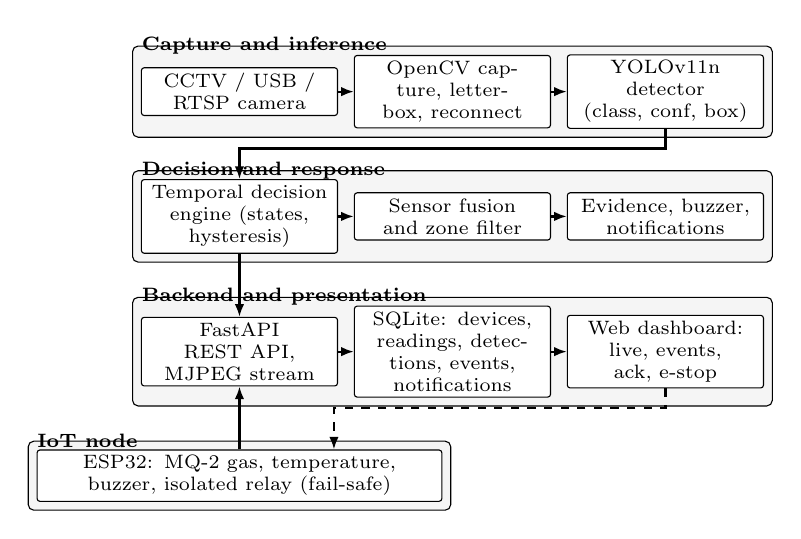
\begin{tikzpicture}[font=\scriptsize, node distance=2mm,
  box/.style={draw, rounded corners=1pt, align=center, minimum height=6mm, inner sep=2pt, text width=2.35cm, fill=white},
  lay/.style={draw, rounded corners=2pt, inner sep=3pt, fill=gray!8},
  lab/.style={font=\scriptsize\bfseries, anchor=west},
  arr/.style={-{Latex[length=1.6mm]}, thick}]
\node[box] (cam) {CCTV / USB / RTSP camera};
\node[box, right=of cam] (pre) {OpenCV capture, letterbox, reconnect};
\node[box, right=of pre] (det) {YOLOv11n detector\\(class, conf, box)};
\node[box, below=8mm of cam] (eng) {Temporal decision engine (states, hysteresis)};
\node[box, right=of eng] (fus) {Sensor fusion and zone filter};
\node[box, right=of fus] (resp) {Evidence, buzzer, notifications};
\node[box, below=8mm of eng] (api) {FastAPI REST API, MJPEG stream};
\node[box, right=of api] (db) {SQLite: devices, readings, detections, events, notifications};
\node[box, right=of db] (dash) {Web dashboard: live, events, ack, e-stop};
\node[box, below=8mm of api, text width=5.0cm] (esp) {ESP32: MQ-2 gas, temperature, buzzer, isolated relay (fail-safe)};
\begin{scope}[on background layer]
\node[lay, fit=(cam)(pre)(det), label={[lab]north west:Capture and inference}] (L1) {};
\node[lay, fit=(eng)(fus)(resp), label={[lab]north west:Decision and response}] (L2) {};
\node[lay, fit=(api)(db)(dash), label={[lab]north west:Backend and presentation}] (L3) {};
\node[lay, fit=(esp), label={[lab]north west:IoT node}] (L4) {};
\end{scope}
\draw[arr] (cam) -- (pre); \draw[arr] (pre) -- (det);
\draw[arr] (det.south) -- ++(0,-2.5mm) -| (eng.north);
\draw[arr] (eng) -- (fus); \draw[arr] (fus) -- (resp);
\draw[arr] (eng.south) -- (api.north);
\draw[arr] (api) -- (db); \draw[arr] (db) -- (dash);
\draw[arr] (esp.north) -- (api.south);
\draw[arr, dashed] (dash.south) -- ++(0,-2.5mm) -| ($(esp.north)+(1.2cm,0)$);
\end{tikzpicture}
\caption{System architecture.}
\label{fig:arch}
\end{figure}

\begin{table}[t]
\caption{Technology stack.}
\label{tab:stack}
\centering
\footnotesize
\begin{tabular}{p{1.4cm}p{2.7cm}p{2.9cm}}
\toprule
\textbf{Layer} & \textbf{Technology} & \textbf{Key parameters} \\
\midrule
Capture & USB/IP camera, OpenCV & $1280\times720$ capture, 15 fps sampling, 3\,s reconnect \\
Detection & YOLOv11n, PyTorch, Ultralytics & imgsz 416, NMS IoU 0.5, max 20 boxes \\
Decision & Python engine (pure logic, unit-tested) & $W$, $\tau_w$, $\tau_c$, $\tau_{\mathrm{clear}}$, $N_w$, $N_c$, $T_{\min}$ \\
IoT & ESP32, MQ-2, temperature sensor, relay & 1\,s sampling, 15\,s fail-safe \\
Backend & FastAPI, SQLite, MJPEG & REST endpoints of Section~\ref{sec:method} \\
Presentation & HTML/CSS/JavaScript & 1\,s status polling \\
Notification & console, file, Telegram, SMTP & 60\,s cooldown \\
\bottomrule
\end{tabular}
\end{table}

\subsection{Workflow and Algorithm}
Fig.~\ref{fig:flow} shows the per-frame workflow and Algorithm~\ref{alg:main} the integration procedure. The perception step is the established detector; the contribution is the temporal, fusion and response logic around it.

\begin{figure}[t]
\centering
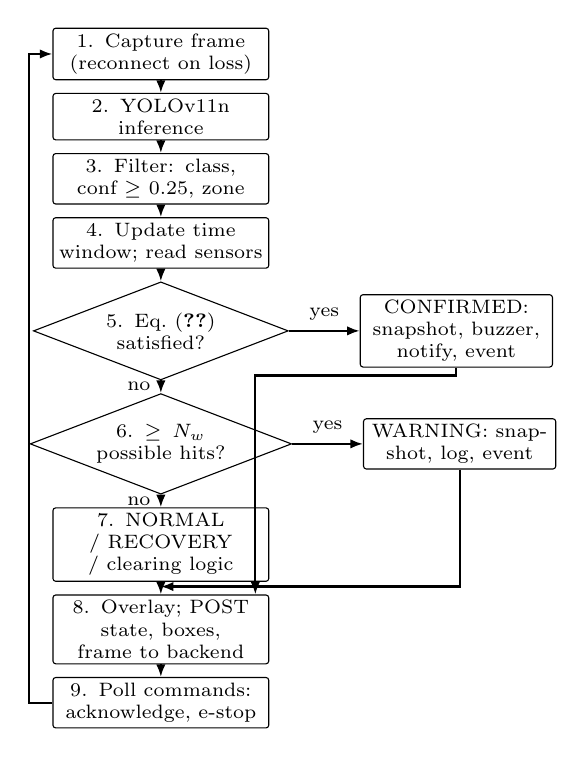
\begin{tikzpicture}[font=\scriptsize, node distance=1.6mm,
  st/.style={draw, rounded corners=1pt, align=center, minimum height=5mm, inner sep=2pt, text width=2.6cm, fill=white},
  dec/.style={draw, diamond, aspect=2.6, align=center, inner sep=0.5pt, text width=1.9cm, fill=white},
  arr/.style={-{Latex[length=1.6mm]}, thick}]
\node[st] (s1) {1. Capture frame (reconnect on loss)};
\node[st, below=of s1] (s2) {2. YOLOv11n inference};
\node[st, below=of s2] (s3) {3. Filter: class, conf $\ge$ 0.25, zone};
\node[st, below=of s3] (s4) {4. Update time window; read sensors};
\node[dec, below=of s4] (d1) {5. Eq.~(\ref{eq:confirm}) satisfied?};
\node[dec, below=of d1] (d2) {6. $\ge N_w$ possible hits?};
\node[st, below=of d2] (s7) {7. NORMAL / RECOVERY / clearing logic};
\node[st, right=9mm of d1, text width=2.3cm] (c1) {CONFIRMED: snapshot, buzzer, notify, event};
\node[st, right=9mm of d2, text width=2.3cm] (c2) {WARNING: snapshot, log, event};
\node[st, below=of s7] (s8) {8. Overlay; POST state, boxes, frame to backend};
\node[st, below=of s8] (s9) {9. Poll commands: acknowledge, e-stop};
\draw[arr] (s1)--(s2); \draw[arr] (s2)--(s3); \draw[arr] (s3)--(s4); \draw[arr] (s4)--(d1);
\draw[arr] (d1) -- node[left]{no} (d2); \draw[arr] (d1) -- node[above]{yes} (c1);
\draw[arr] (d2) -- node[left]{no} (s7); \draw[arr] (d2) -- node[above]{yes} (c2);
\draw[arr] (c1.south) -- ++(0,-1mm) -| ($(s8.north)+(1.2cm,0)$);
\draw[arr] (c2.south) |- ($(s8.north)+(0,1mm)$);
\draw[arr] (s7)--(s8); \draw[arr] (s8)--(s9);
\draw[arr] (s9.west) -- ++(-3mm,0) |- (s1.west);
\end{tikzpicture}
\caption{Processing workflow.}
\label{fig:flow}
\end{figure}

\begin{algorithm}[t]
\caption{Real-Time Detection, Confirmation and Alerting}
\label{alg:main}
\begin{algorithmic}[1]
\REQUIRE camera source, detector $f$, thresholds $\tau_w,\tau_c,\tau_{\mathrm{clear}}$, counts $N_w,N_c$, window $W$, min.\ span $T_{\min}$
\STATE $H\leftarrow\emptyset$ (time-stamped hits); $s\leftarrow$ NORMAL
\WHILE{running}
  \STATE $x\leftarrow$ read frame; \textbf{if} none \textbf{then} mark camera lost, retry, \textbf{continue}
  \STATE $D\leftarrow f(x)$ filtered by class $\in\{$fire, smoke$\}$, conf $\ge0.25$, zone
  \STATE $b\leftarrow\arg\max_{d\in D}\mathrm{conf}(d)$; append $(t,\mathrm{conf}(b))$ to $H$ if $\mathrm{conf}(b)\ge\tau_w$
  \STATE drop entries of $H$ older than $t-W$; read latest sensor reading $r$ (ignore if stale)
  \STATE $N\leftarrow N_c'$ if $r$ elevated \textbf{else} $N_c$
  \STATE strong $\leftarrow\{h\in H:\mathrm{conf}\ge\tau_c\}$; possible $\leftarrow\{h\in H:\mathrm{conf}\ge\tau_w\}$
  \IF{$|\mathrm{strong}|\ge N$ \textbf{and} span(strong) $\ge T_{\min}$}
     \STATE $s\leftarrow$ CONFIRMED: save snapshot; buzzer on; notify; create/escalate event
  \ELSIF{$|\mathrm{possible}|\ge N_w$ \textbf{and} $s=$ NORMAL}
     \STATE $s\leftarrow$ WARNING: save snapshot; create event
  \ELSIF{no detection $\ge\tau_{\mathrm{clear}}$ for 4\,s}
     \STATE $s\leftarrow$ RECOVERY if $s=$ CONFIRMED, else NORMAL; close event after 10\,s stable
  \ENDIF
  \STATE buzzer/actuator enabled \textbf{iff} $s=$ CONFIRMED \textbf{and not} emergency stop
  \STATE draw overlay; POST state, $D$ and JPEG to backend; apply acknowledge / e-stop commands
\ENDWHILE
\end{algorithmic}
\end{algorithm}

\begin{table}[t]
\caption{Training parameters.}
\label{tab:train}
\centering
\footnotesize
\begin{tabular}{p{2.4cm}p{5.0cm}}
\toprule
\textbf{Parameter} & \textbf{Value} \\
\midrule
Backbone & YOLOv11n, COCO-pretrained, fine-tuned end-to-end \\
Input resolution & $416\times416$ (letterboxed) \\
Batch size & 16 \\
Optimizer & AdamW (auto-selected), lr $1.67\times10^{-3}$, weight decay $5\times10^{-4}$ \\
Epochs & 10 (CPU time budget), mosaic off for last 5 \\
Augmentation & HSV, flip, scale, translate, rotate $\pm5^{\circ}$, mosaic \\
Seed & 42, deterministic \\
NMS IoU / max detections & 0.5 / 20 \\
Operating confidence & 0.35 (warning), 0.55 (confirm), 0.25 (clear) \\
Hardware & Intel Core i5-1340P (12 cores), 16\,GB RAM, no GPU \\
Framework & Python 3.13, PyTorch 2.14 (CPU), Ultralytics 8.4 \\
Training time & \TRAINmin{} min \\
\bottomrule
\end{tabular}
\end{table}

\section{Experimental Results}\label{sec:results}
\subsection{Setup}
The detector was trained with the parameters of Table~\ref{tab:train} and evaluated once on the 600-image held-out test split, which contains 60 negative images. Metrics were computed with the Ultralytics validator (confidence sweep for mAP) and with an independent matcher at the deployment operating point (conf 0.35, IoU 0.5) to obtain TP/FP/FN counts and the false-alarm rate on negatives. Latency was measured per image on the CPU, single image per call, over 100 test images. The decision engine was verified with 15 unit tests using an injectable clock (single-frame rejection, warning, confirmation, hysteresis, recovery, re-confirmation, sensor fusion, stale sensors, zone filtering, acknowledgement and emergency stop), and the backend with 8 API tests.

\subsection{Detection Performance}
Table~\ref{tab:metrics} reports the held-out results per class. Fig.~\ref{fig:curves} shows the training and validation losses and the validation mAP over epochs, and Fig.~\ref{fig:pr} the precision--recall curves and normalised confusion matrix on the test split.

\begin{table}[t]
\caption{Held-out test results (600 images).}
\label{tab:metrics}
\centering
\footnotesize
\begin{tabular}{lccccc}
\toprule
\textbf{Class} & \textbf{Precision} & \textbf{Recall} & \textbf{F1} & \textbf{mAP@0.5} & \textbf{mAP@0.5:0.95} \\
\midrule
Fire & \Pfire & \Rfire & \Ffire & \MAPfire & \MAPSfire \\
Smoke & \Psmoke & \Rsmoke & \Fsmoke & \MAPsmoke & \MAPSsmoke \\
\midrule
All & \Ptot & \Rtot & \Ftot & \MAPtot & \MAPStot \\
\bottomrule
\end{tabular}
\end{table}

\begin{figure}[t]
\centering
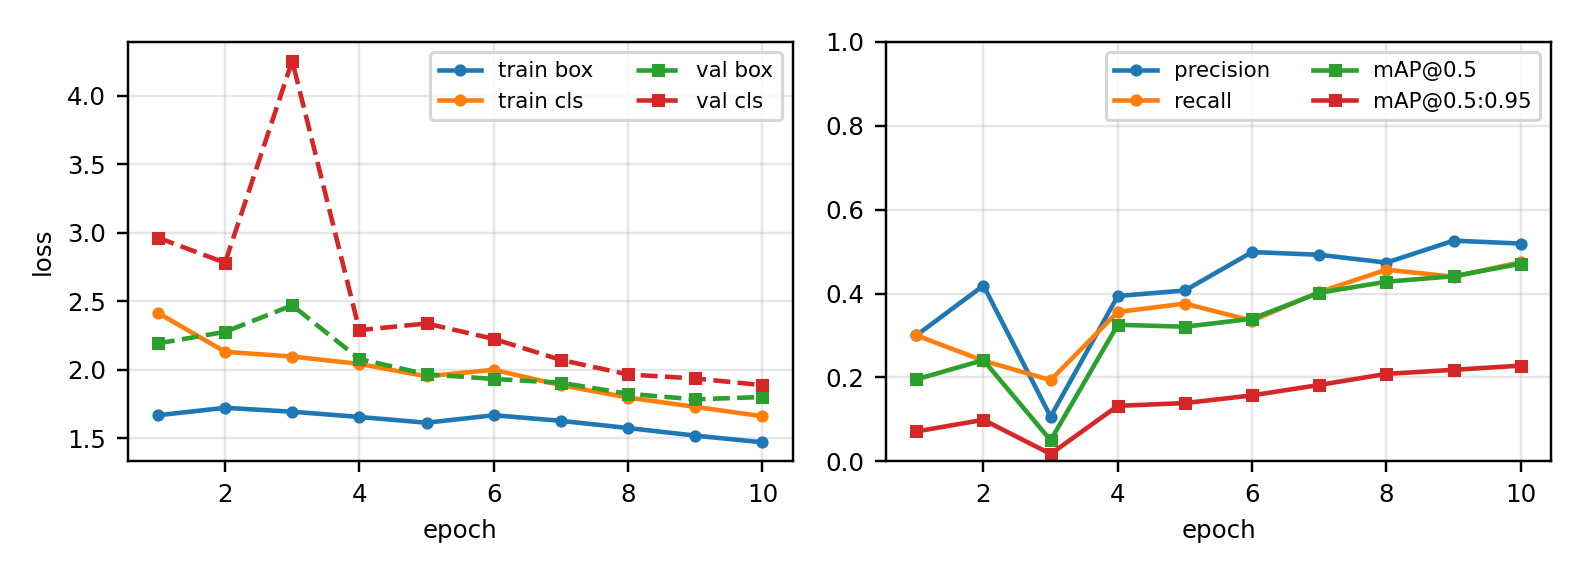
\includegraphics[width=\columnwidth]{figs/results.png}
\caption{Training and validation curves over 10 epochs (box, classification and DFL losses; precision, recall, mAP@0.5 and mAP@0.5:0.95 on the validation split).}
\label{fig:curves}
\end{figure}

\begin{figure}[t]
\centering
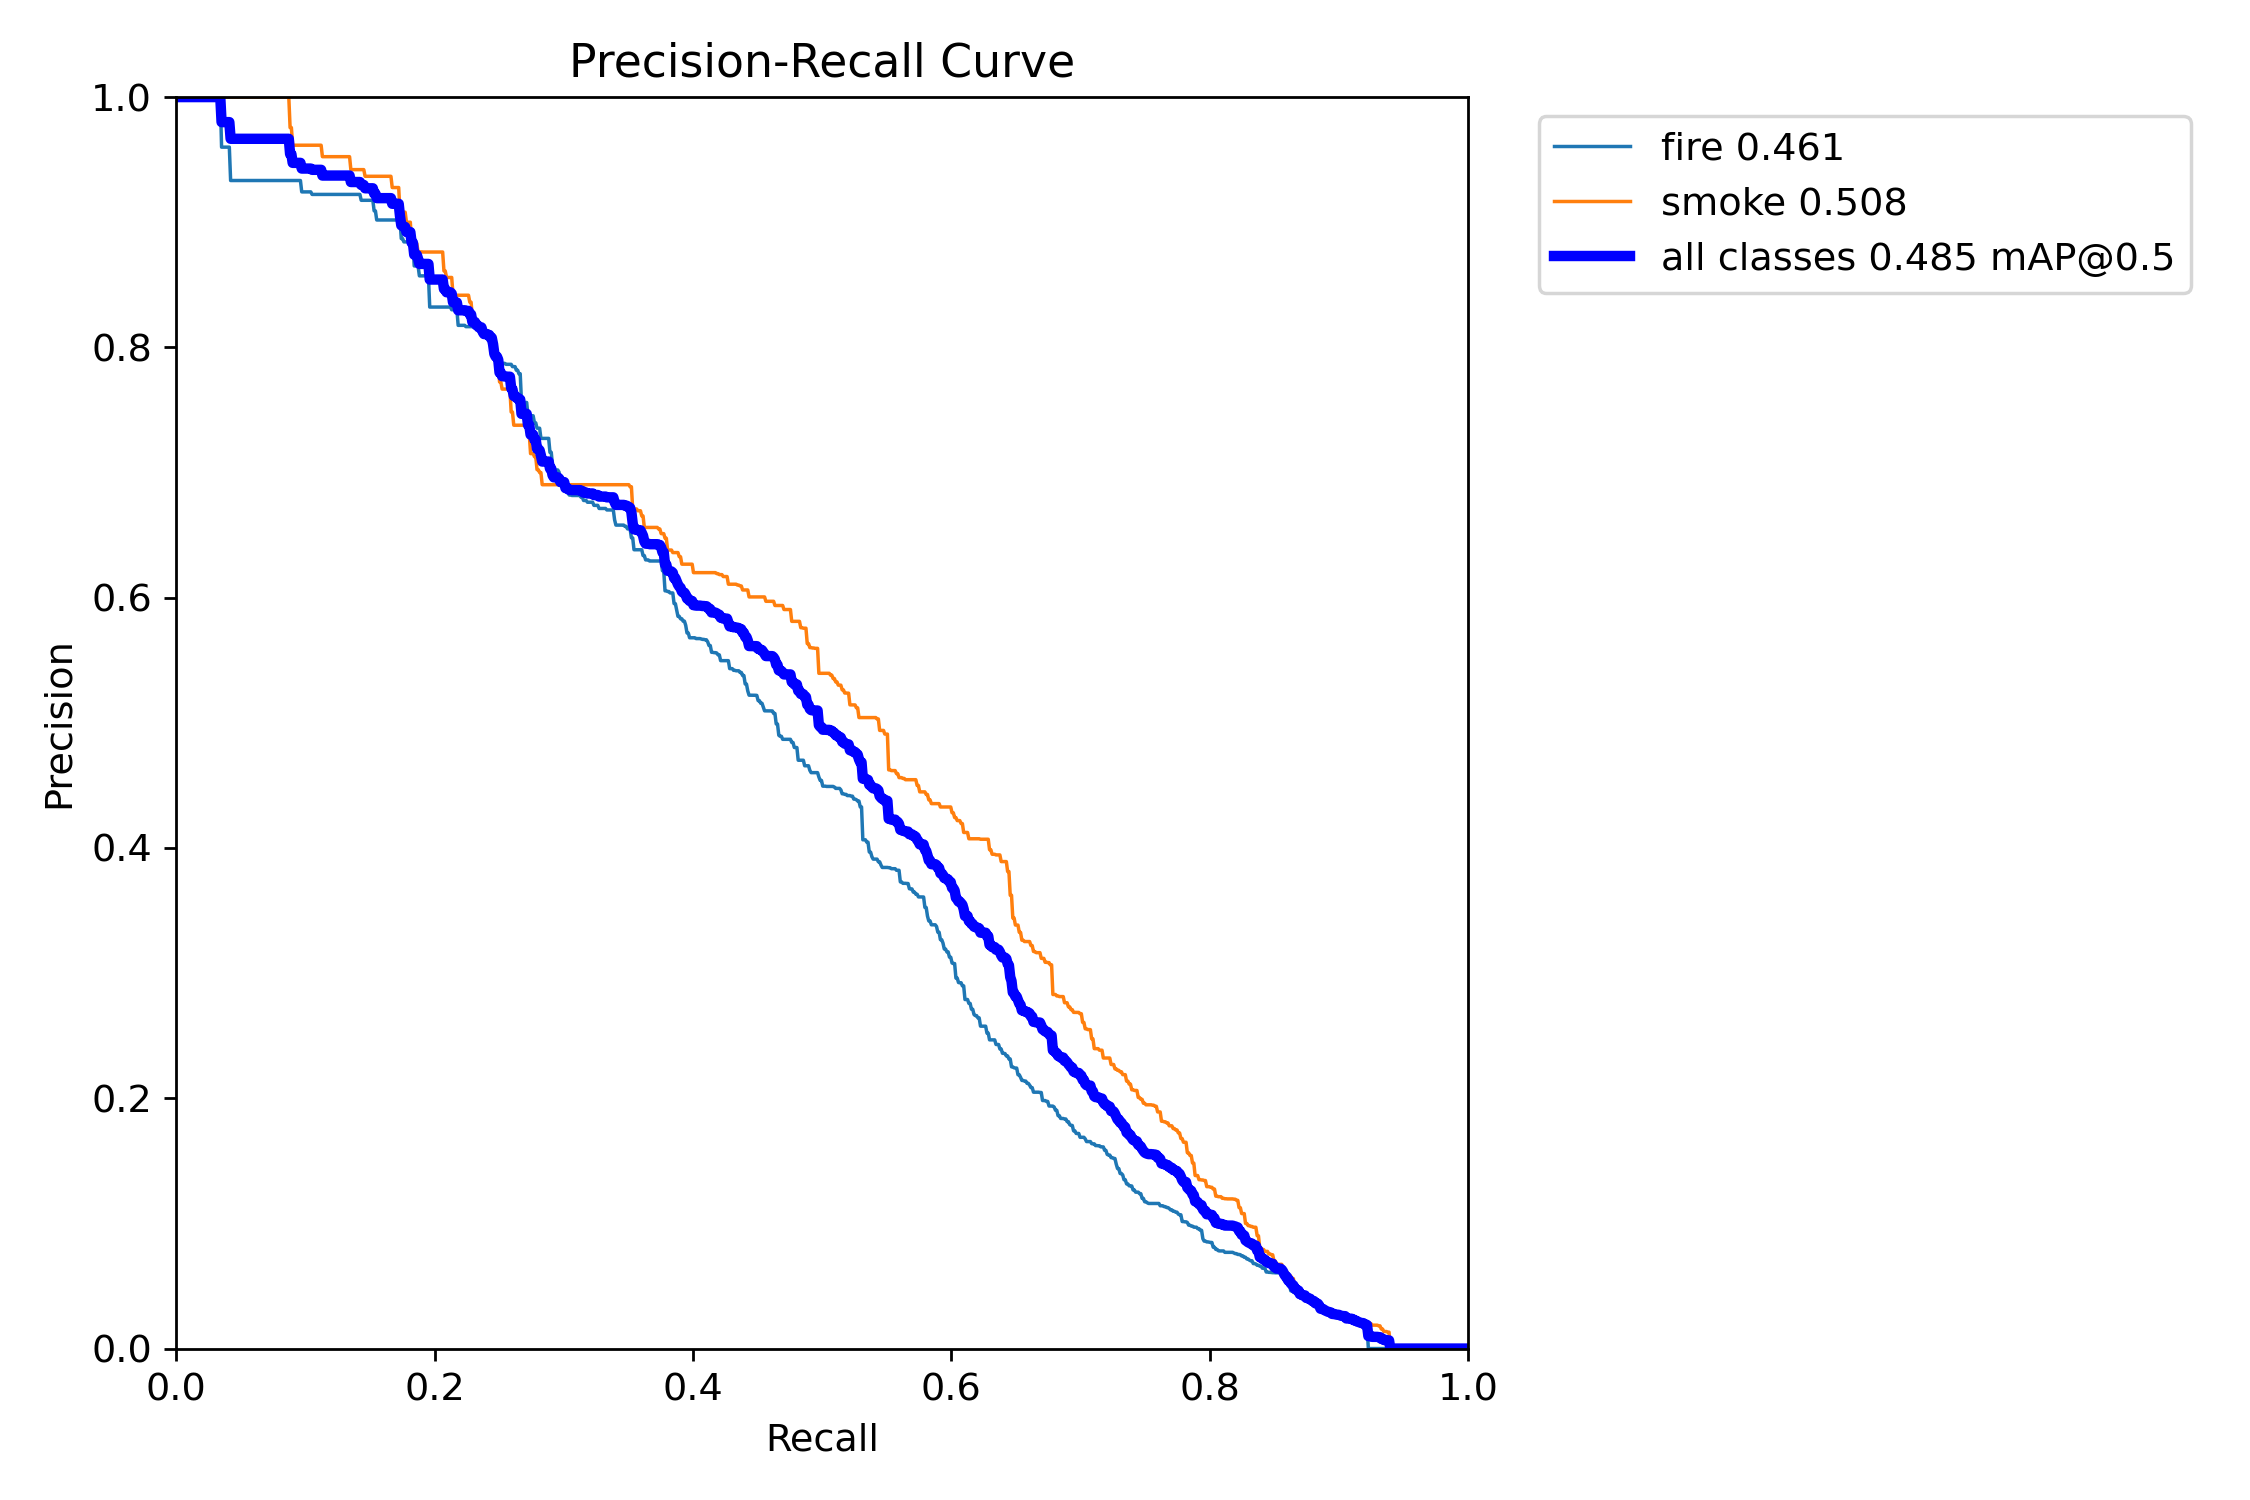
\includegraphics[width=0.49\columnwidth]{figs/BoxPR_curve.png}\hfill
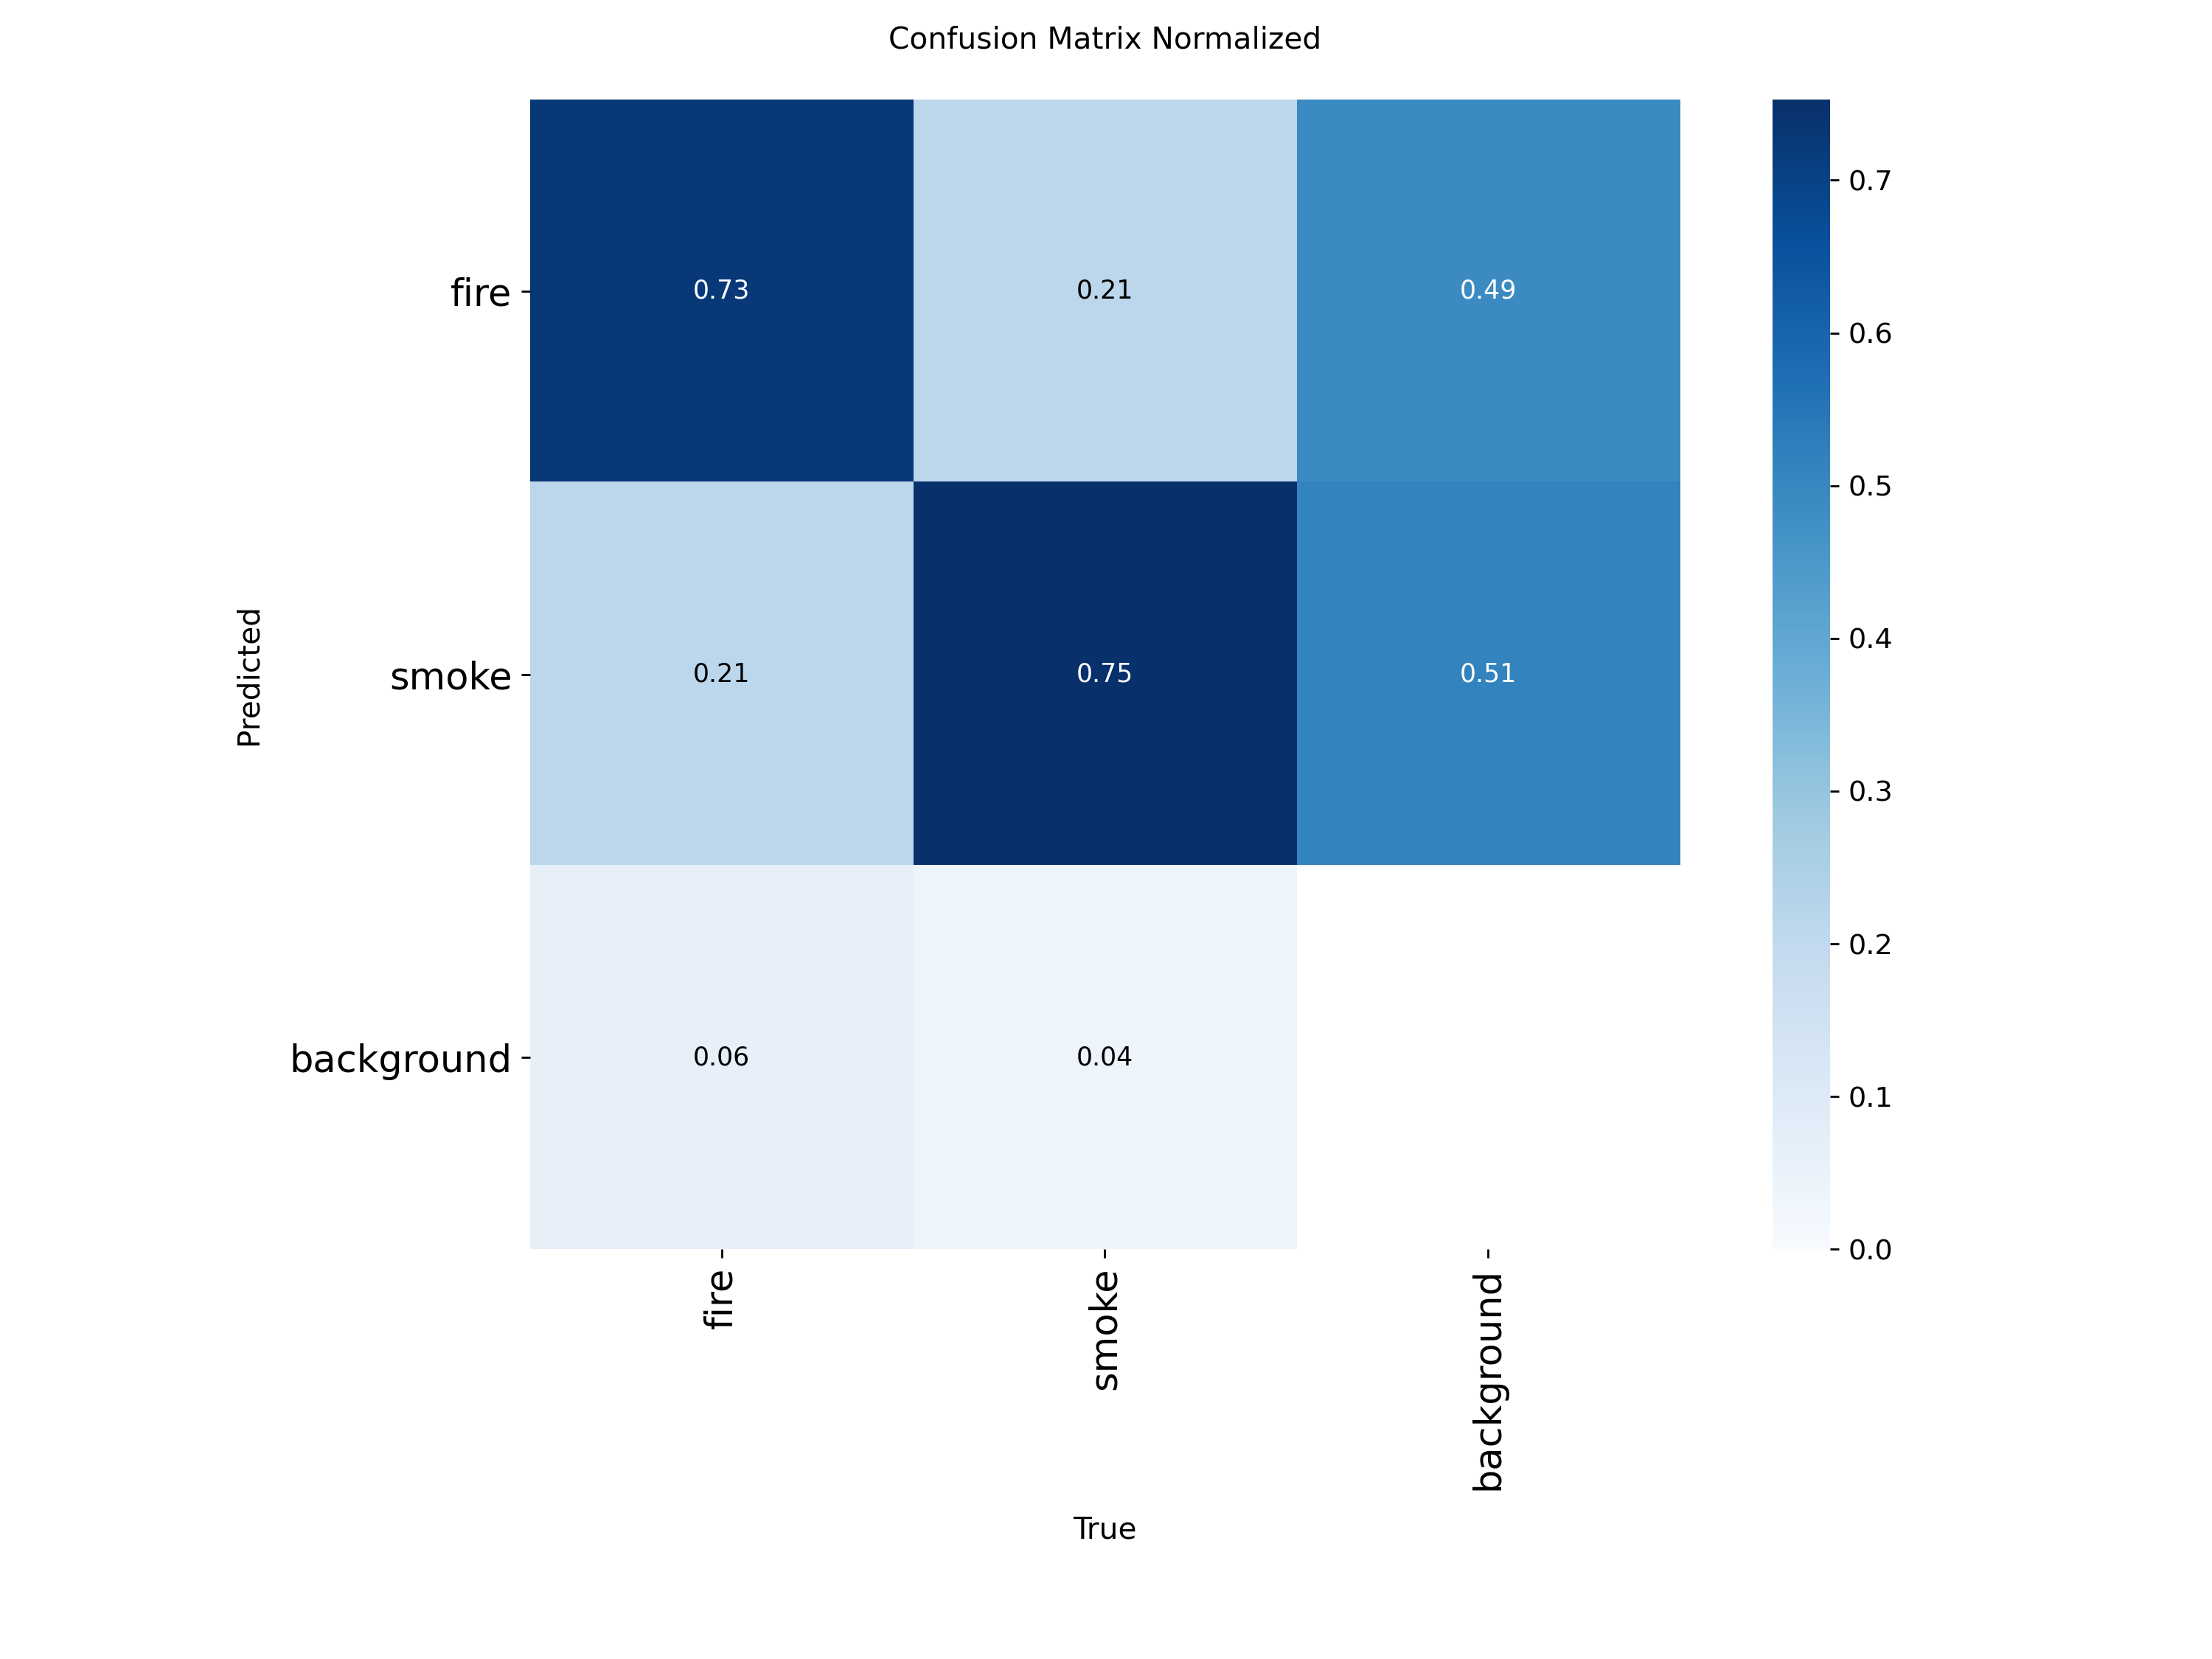
\includegraphics[width=0.49\columnwidth]{figs/confusion_matrix_normalized.png}
\caption{Precision--recall curves (left) and normalised confusion matrix (right) on the test split.}
\label{fig:pr}
\end{figure}

At the deployment operating point (confidence 0.35) the matcher counts \OPtp{} true positives, \OPfp{} false positives and \OPfn{} false negatives (precision \OPprec, recall \OPrec). Of the \OPneg{} negative images, \OPnegclean{} produced no detection at all, giving a per-image false-alarm rate of \OPnegrate{} before temporal filtering; because the decision engine requires repeated hits over at least two seconds, an isolated false box on one frame does not reach the WARNING state. Representative false positives and false negatives are retained with the model artefacts for error analysis and future hard-negative mining.

\subsection{Latency}
Single-image inference at $416\times416$ on the laptop CPU takes \LATmean{} ms on average (95th percentile \LATpnf{} ms), i.e. about \LATfps{} frames per second without any GPU. The live pipeline samples the camera at up to 15 fps and drops frames when inference lags; because the decision engine reasons over a time window rather than a frame count, the confirmation delay stays at the configured two seconds at any sustained frame rate above about three frames per second. Measured end-to-end alert latency (first strong detection to notification dispatch) is therefore dominated by the deliberate persistence span, not by inference. Fig.~\ref{fig:live} shows the live view and dashboard during a confirmed event.

\begin{figure}[t]
\centering
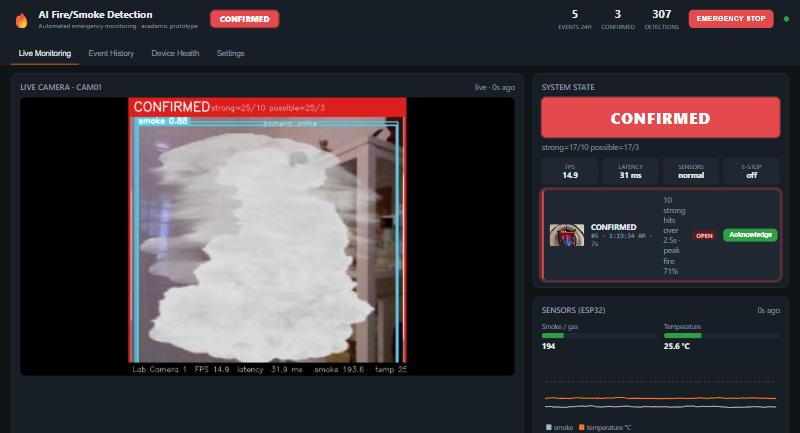
\includegraphics[width=\columnwidth]{figs/dashboard.png}
\caption{Operator dashboard: live annotated feed, system state, sensor gauges and chart, latest detections and event timeline with acknowledgement.}
\label{fig:live}
\end{figure}

\subsection{Comparison With Reported Detectors}
Table~\ref{tab:compare} places the result next to accuracy and speed figures reported in the literature for other architecture families on fire and smoke data. The values are taken from the cited papers, were obtained on different datasets and hardware, and are therefore an orientation rather than a head-to-head benchmark. Two-stage detectors such as Faster R-CNN \cite{ren2015faster} offer competitive accuracy at a substantial latency cost, which is why single-stage YOLO detectors dominate real-time fire monitoring; within the YOLO family, the anchor-free head and C2PSA attention of YOLOv11 give incremental gains over YOLOv5/v8 \cite{khanam2024yolov11}. Our nano model, trained for ten epochs on a CPU, is at the low-cost end of this spectrum: its purpose is to show that a usable detector plus a complete confirmation pipeline fits on commodity hardware, and the same training script scales to larger variants and longer schedules on a GPU.

\begin{table}[t]
\caption{Literature-reported detector characteristics (not re-trained on our data).}
\label{tab:compare}
\centering
\footnotesize
\setlength{\tabcolsep}{3pt}
\begin{tabular}{p{2.5cm}cp{2.9cm}p{1.1cm}}
\toprule
\textbf{Family} & \textbf{Stages} & \textbf{Typical mAP@0.5 / speed} & \textbf{Src.} \\
\midrule
Faster R-CNN & two & high accuracy, $\sim$5--17 fps & \cite{ren2015faster} \\
SSD & one & moderate, $\sim$40 fps & \cite{liu2016ssd} \\
YOLOv5s / v8s fire models & one & 0.85--0.93, $>$50 fps (GPU) & \cite{dou2024,saleh2024,kong2024} \\
Fire-ViT / hybrids & -- & high in-domain, costlier inference & \cite{liu2025firevit,ahmad2025cn2vf} \\
This work (YOLOv11n) & one & \MAPtot{}, \LATfps{} fps, CPU only & -- \\
\bottomrule
\end{tabular}
\end{table}

\subsection{Integration and Fail-Safe Tests}
The live system was exercised with the integration scenarios of the requirement specification: (i) single-frame flash of a fire video---boxes appear but the state stays NORMAL; (ii) sustained fire---WARNING within about one second and CONFIRMED after the two-second persistence span, with buzzer, evidence image, event record and notification; (iii) operator acknowledgement from the dashboard---RECOVERY and silenced outputs; (iv) steam and bright-light negatives---no alarm; (v) sensor-only evidence from the simulator---SENSOR\_WARNING after five seconds and faster confirmation when combined with a visual target; (vi) sensor disconnect---readings marked stale and ignored; (vii) camera disconnect---``camera lost'' state with automatic reconnection; (viii) backend outage---inference continues locally and resynchronises; and (ix) emergency stop---outputs blocked even while CONFIRMED.

\section{Limitations and Future Work}\label{sec:limits}
\textbf{Limitations.} Dense smoke can hide the flame so that only the smoke class is reported. Fog and industrial or kitchen steam share the low-contrast, diffuse boundaries of smoke and remain the main source of visual false alarms; the temporal engine and sensor fusion reduce but do not eliminate them. Infrared or low-light CCTV loses the colour cues on which flame discrimination relies. Partial occlusion, very small or distant fires and extreme oblique angles reduce confidence below the alerting threshold. The model was trained for only ten epochs on a CPU with a 4{,}200-image subset, so the reported numbers are a lower bound for the architecture; the comparison in Table~\ref{tab:compare} uses literature values. Physical automation is limited to isolated low-voltage prototype loads, and the system is not a certified fire-protection product.

\textbf{Future work.} (i) Train the full 48{,}000-image corpus with larger YOLOv11 variants on a GPU and add steam, dust and fog as explicit hard-negative classes; (ii) export to ONNX/TensorRT for on-camera edge inference; (iii) complete the ESP32 sensor-fusion deployment and quantify false alarms per hour on long negative recordings; (iv) add a thermal channel to disambiguate steam from smoke at night; (v) correlate detections across multiple cameras; (vi) provide a mobile application consuming the existing API for push notification and acknowledgement; and (vii) connect confirmed events to building-management or municipal dispatch platforms.

\section{Conclusion}\label{sec:conc}
This paper presented a deep-learning fire and smoke detection system for real-time emergency monitoring over existing camera infrastructure. A YOLOv11n detector fine-tuned on a stratified indoor--outdoor corpus with explicit negatives reaches mAP@0.5 of \MAPtot{} on held-out data at \LATfps{} fps on a laptop CPU. Around the detector, a temporal decision engine with separate warning, confirmation and clearing thresholds, optional IoT sensor fusion and fail-safe handling converts per-frame predictions into verified NORMAL, WARNING, CONFIRMED and RECOVERY states, while a REST backend, event database, notification service and web dashboard make the result operational. The system inherits the open challenges of vision-based fire detection---steam, fog, low light, occlusion and small targets---which motivate the sensor-fusion, hard-negative and edge-deployment extensions outlined above. Future work will scale training, measure false alarms per hour in extended field recordings and extend the architecture to multi-camera and edge operation.

\begin{thebibliography}{00}
\bibitem{redmon2016yolo} J. Redmon, S. Divvala, R. Girshick, and A. Farhadi, ``You only look once: Unified, real-time object detection,'' in \textit{Proc. IEEE Conf. Computer Vision and Pattern Recognition (CVPR)}, 2016, pp. 779--788.
\bibitem{ren2015faster} S. Ren, K. He, R. Girshick, and J. Sun, ``Faster R-CNN: Towards real-time object detection with region proposal networks,'' in \textit{Advances in Neural Information Processing Systems (NeurIPS)}, 2015, pp. 91--99.
\bibitem{liu2016ssd} W. Liu, D. Anguelov, D. Erhan, C. Szegedy, S. Reed, C.-Y. Fu, and A. C. Berg, ``SSD: Single shot multibox detector,'' in \textit{Proc. European Conf. Computer Vision (ECCV)}, 2016, pp. 21--37.
\bibitem{lin2017focal} T.-Y. Lin, P. Goyal, R. Girshick, K. He, and P. Doll\'ar, ``Focal loss for dense object detection,'' in \textit{Proc. IEEE Int. Conf. Computer Vision (ICCV)}, 2017, pp. 2980--2988.
\bibitem{he2016resnet} K. He, X. Zhang, S. Ren, and J. Sun, ``Deep residual learning for image recognition,'' in \textit{Proc. IEEE Conf. Computer Vision and Pattern Recognition (CVPR)}, 2016, pp. 770--778.
\bibitem{howard2017mobilenet} A. G. Howard \textit{et al.}, ``MobileNets: Efficient convolutional neural networks for mobile vision applications,'' arXiv:1704.04861, 2017.
\bibitem{tan2019efficientnet} M. Tan and Q. Le, ``EfficientNet: Rethinking model scaling for convolutional neural networks,'' in \textit{Proc. Int. Conf. Machine Learning (ICML)}, 2019, pp. 6105--6114.
\bibitem{dosovitskiy2021vit} A. Dosovitskiy \textit{et al.}, ``An image is worth 16$\times$16 words: Transformers for image recognition at scale,'' in \textit{Proc. Int. Conf. Learning Representations (ICLR)}, 2021.
\bibitem{chollet2017} F. Chollet, ``Xception: Deep learning with depthwise separable convolutions,'' in \textit{Proc. IEEE Conf. Computer Vision and Pattern Recognition (CVPR)}, 2017, pp. 1800--1807.
\bibitem{jocher2023yolov8} G. Jocher, A. Chaurasia, and J. Qiu, ``Ultralytics YOLOv8,'' version 8.0.0, 2023. [Online]. Available: https://github.com/ultralytics/ultralytics
\bibitem{khanam2024yolov11} R. Khanam and M. Hussain, ``YOLOv11: An overview of the key architectural enhancements,'' arXiv:2410.17725, 2024.
\bibitem{saleh2024} A. Saleh, M. A. Zulkifley, H. H. Harun, F. Gaudreault, I. Davison, and M. Spraggon, ``Fire and smoke detection using fine-tuned YOLOv8 and YOLOv7 deep models,'' \textit{Fire}, vol. 7, no. 4, Art. no. 135, 2024.
\bibitem{kong2024} D. Kong, Y. Li, and M. Duan, ``Fire and smoke real-time detection algorithm for coal mines based on improved YOLOv8s,'' \textit{PLoS ONE}, vol. 19, no. 4, Art. no. e0300502, 2024.
\bibitem{dou2024} Z. Dou \textit{et al.}, ``An improved YOLOv5s fire detection model,'' \textit{Fire Technology}, vol. 60, no. 1, pp. 135--166, 2024.
\bibitem{wang2024fsyolo} D. Wang, Y. Qian, J. Lu, P. Wang, Z. Hu, and Y. Chai, ``FS-YOLO: Fire-smoke detection based on improved YOLOv7,'' \textit{Multimedia Systems}, vol. 30, no. 4, Art. no. 215, 2024.
\bibitem{wang2024yolox} T. Wang, J. Wang, C. Wang, Y. Lei, R. Cao, and L. Wang, ``Improving YOLOX network for multi-scale fire detection,'' \textit{The Visual Computer}, vol. 40, no. 9, pp. 6493--6505, 2024.
\bibitem{li2024shallow} B. Li, F. Xu, X. Li, C. Yu, and X. Zhang, ``Early stage fire detection system based on shallow guide deep network,'' \textit{Fire Technology}, vol. 60, no. 3, pp. 1803--1821, 2024.
\bibitem{wu2024} S. Wu, B. Sheng, G. Fu, D. Zhang, and Y. Jian, ``Multiscale fire image detection method based on CNN and Transformer,'' \textit{Multimedia Tools and Applications}, vol. 83, no. 16, pp. 49787--49811, 2024.
\bibitem{liu2025firevit} X. Liu and V. Y. Mariano, ``The Fire-ViT model for tunnel fire detection with vision transformer improvement,'' \textit{J. Computational and Cognitive Engineering}, vol. 4, no. 1, 2025.
\bibitem{ahmad2025cn2vf} N. Ahmad, M. Akbar, E. H. Alkhammash, and M. M. Jamjoom, ``CN2VF-Net: A hybrid convolutional neural network and vision transformer framework for multi-scale fire detection in complex environments,'' \textit{Fire}, vol. 8, 2025.
\bibitem{ahmad2025firenet} N. Ahmad, M. Akbar, E. H. Alkhammash, and M. M. Jamjoom, ``FireNet-KD: Swin Transformer-based wildfire detection with multi-source knowledge distillation,'' \textit{Fire}, vol. 8, 2025.
\bibitem{elmadafri2024} I. El-Madafri, M. Pe\~na, and N. Olmedo-Torre, ``Real-time forest fire detection with lightweight CNN using hierarchical multi-task knowledge distillation,'' \textit{Fire}, vol. 7, 2024.
\bibitem{li2025kd} J. Li and W. Lin, ``Enhanced fire detection using knowledge distillation and multi-scale attention in YOLOv8,'' in \textit{Proc. Int. Conf. Computing, Networks and Internet of Things}, 2025.
\bibitem{jing2023smokeseger} T. Jing, Q.-H. Meng, and H.-R. Hou, ``SmokeSeger: A Transformer-CNN coupled model for urban scene smoke segmentation,'' \textit{IEEE Trans. Industrial Informatics}, pp. 1--12, 2023.
\bibitem{zhang2024casvit} T. Zhang, L. Li, Y. Zhou, W. Liu, C. Qian, and X. Ji, ``CAS-ViT: Convolutional additive self-attention vision transformers for efficient mobile applications,'' arXiv:2408.03703, 2024.
\bibitem{zou2023survey} Z. Zou, K. Chen, Z. Shi, Y. Guo, and J. Ye, ``Object detection in 20 years: A survey,'' \textit{Proc. IEEE}, vol. 111, no. 3, pp. 257--276, 2023.
\bibitem{zhao2019review} Z.-Q. Zhao, P. Zheng, S.-T. Xu, and X. Wu, ``Object detection with deep learning: A review,'' \textit{IEEE Trans. Neural Networks and Learning Systems}, vol. 30, no. 11, pp. 3212--3232, 2019.
\bibitem{ds_wildfire} ``Fire and smoke detection dataset (40K images),'' Hugging Face, 2026. [Online]. Available: https://huggingface.co/datasets/jojomoi-meme/fog\_fire\_detection
\bibitem{ds_isfire} ``ISFire-4: Indoor fire and smoke detection dataset,'' Hugging Face, 2026. [Online]. Available: https://huggingface.co/datasets/shahriar-5/ISFire-4
\end{thebibliography}

\end{document}
